%!TEX TS-program = xelatex
\documentclass[]{friggeri-cv}
\usepackage{afterpage}
\usepackage{hyperref}
\usepackage{color}
\usepackage[normalem]{ulem}
\usepackage{xcolor}
\hypersetup{
    pdftitle={},
    pdfauthor={},
    pdfsubject={},
    pdfkeywords={},
    colorlinks=false,       % no lik border color
   allbordercolors=white    % white border color for all
}
\addbibresource{bibliography.bib}
\RequirePackage{xcolor}
\definecolor{pblue}{HTML}{0395DE}

\makeatletter
\let\old@rule\@rule
\def\@rule[#1]#2#3{\textcolor{rulecolor}{\old@rule[#1]{#2}{#3}}}
\makeatother

\definecolor{rulecolor}{named}{gray}

\begin{document}
\header{Vincent}{Castelluci}
      {Full stack developer}
\hfill \lq\textit{Do, fail, improve}\rq

\rule{397pt}{8pt}

% In the aside, each new line forces a line break
\begin{aside}
  \section{Address}
  \hspace{1cm}
    19 rue de Thizy
    69470, Cours-la-ville
    France
  \section{Contacts}
  \hspace{1cm}
    
\includegraphics[scale=0.60]{img/france.png}~\href{tel:+33634321575}{+336 3432 1575}
    
\includegraphics[scale=0.60]{img/thailand.png}~\href{tel:+66910217942}{+669 1021 7942}
    \hspace{-2cm}\href{mailto:vincent.castelluci@gmail.com}{
\includegraphics[scale=0.60]{img/mail.png}~vincent@castelluci.xyz}
    \href{https://www.linkedin.com/in/vincent-castelluci-363939170}{
\includegraphics[scale=0.60]{img/linkedin.png}~vincent-castelluci}
    \href{skype://vincent690022?userinfo}{
\includegraphics[scale=0.60]{img/skype.png}~vincent690022}
    ~
  \section{Technical}
  \hspace{1cm}
    \textbf{Learning}
\includegraphics[scale=0.40]{img/5puces.png}
    \textbf{Java}
\includegraphics[scale=0.40]{img/5puces.png}
    \textbf{TDD}
\includegraphics[scale=0.40]{img/5puces.png}
    \textbf{JavaScript}
\includegraphics[scale=0.40]{img/4puces.png}
    \textbf{HTML}
\includegraphics[scale=0.40]{img/4puces.png}
    \textbf{CSS}
\includegraphics[scale=0.40]{img/3puces.png}
    \textbf{Python}
\includegraphics[scale=0.40]{img/2puces.png}
    \textbf{Spring}
\includegraphics[scale=0.40]{img/4puces.png}
    \textbf{Pipelines}
\includegraphics[scale=0.40]{img/5puces.png}
    \textbf{Git}
\includegraphics[scale=0.40]{img/4puces.png}
    \textbf{Maven}
\includegraphics[scale=0.40]{img/4puces.png}
    \textbf{Docker}
\includegraphics[scale=0.40]{img/3puces.png}
    \textbf{SQL}
\includegraphics[scale=0.40]{img/3puces.png}
    \textbf{GNU/Linux}
\includegraphics[scale=0.40]{img/4puces.png}
    \textbf{Windows}
\includegraphics[scale=0.40]{img/3puces.png}
    ~
  \section{Personal Skills}
  \hspace{1cm}
    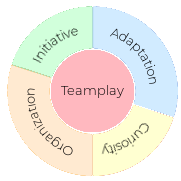
\includegraphics[scale=0.62]{img/personal.png}
    ~
  \section{Languages}
  \hspace{1cm}
    \textbf{French}
\includegraphics[scale=0.40]{img/5puces.png}
    \textbf{English}
\includegraphics[scale=0.40]{img/4puces.png}
    \textbf{Thai}
\includegraphics[scale=0.40]{img/2puces.png}
    \textbf{German}
\includegraphics[scale=0.40]{img/2puces.png}
\end{aside}

\section{Summary}
Experienced Java fullstack developer with a great concern for results and quality.\\
I love to learn, apply and research on my own new solutions to improve lifecycle and quality of my projects.\\
My past experiences taught me many things, but the most important one is that the only way to succeed is to try, fail and improve, which is the reason I love to use TDD methodology.\\
Ideally looking for challenging missions in fields I am not yet comfortable with or I don't even know, with high expectations on quality and results, either remotely or on site.\\
\textbf{What I am not looking for :}
\begin{itemize}
\item Team who does not understand the value of TDD
\vspace{-\baselineskip}
\vspace{1 ex}
\item Team where human qualities are not the central key to success
\vspace{-\baselineskip}
\vspace{1 ex}
\item Team following others methodologies without adding adapation or cleverness
\vspace{-\baselineskip}
\vspace{1 ex}
\item Team who keeps doing the same mistakes without will to improve
\end{itemize}

\section{Experiences}
\begin{entrylist}
  \entry
    {07/18 - Now}
    {Full stack developer}
    {Freelance, Remote, Worldwide}
    {Currently in development for my own project, I am becoming much more familiar with all modern DevOps tools such as AWS, Kubernetes, BitBucket and its ecosystem,... as well as with modern frontend tools such as React.js, Bulma and SASS.\\}
    \entry
    {06/16 - 07/18}
    {Lead full stack developer}
    {Ubik Ingénierie for Decathlon E-Commerce, France}
    {
My main tasks were to :
      \begin{itemize}
        \item improve quality of the payment perimeter through code reviews, tests, spreading best practices, upgrading frameworks and API...
        \item train newcomers to be operational as quickly as possible by redacting documentation on processes, plan training, pair programming and mob programming sessions
        \item open the application source (which is not as easy as it seems as it points out many flaws, severe or minor)
        \item make the application more robust and resilient by adding stress tests, measure health and plan emergency solutions in urgent cases
      \end{itemize}
}
    \entry
    {06/14 - 06/16}
    {Full stack developer}
    {Ubik Ingénierie for Decathlon E-Commerce, France}
    {My main mission was to maintain, improve and support the centralised payment middleware as well as integrate it on the European Decathlon website.\\
When I arrived, we were starting to move toward agile methodologies and it has been a long and interesting voyage, which never ends as continuous improvement was and still is my motto.\\}
\end{entrylist}

\section{Passions}

\includegraphics[scale=0.6]{img/books.png}\hspace{2.4 em}
\includegraphics[scale=0.6]{img/team.png}\hspace{2.4 em}
\includegraphics[scale=0.6]{img/programming.png}\hspace{2.4 em}
\includegraphics[scale=0.6]{img/chess.png}\hspace{2.4 em}
\includegraphics[scale=0.6]{img/formula.png}
\phantom{}\hspace{2 em}Books\hspace{4.2 em}Team sports\hspace{4.2 em}Coding\hspace{3.6 em}Strategy games\hspace{2.2 em}Mathematics

%%% This piece of code has been commented by Karol Kozioł due to biblatex errors. 
% 
%\printbibsection{article}{article in peer-reviewed journal}
%\begin{refsection}
%  \nocite{*}
%  \printbibliography[sorting=chronological, type=inproceedings, title={international peer-reviewed conferences/proceedings}, notkeyword={france}, heading=subbibliography]
%\end{refsection}
%\begin{refsection}
%  \nocite{*}
%  \printbibliography[sorting=chronological, type=inproceedings, title={local peer-reviewed conferences/proceedings}, keyword={france}, heading=subbibliography]
%\end{refsection}
%\printbibsection{misc}{other publications}
%\printbibsection{report}{research reports}

\end{document}